\documentclass[c]{beamer}
\usepackage{org-preamble}
\usepackage[cpp_teaching]{slide-style}
\usepackage{minted}
\newcommand{\inline}[1]{\mintinline[breaklines]{c++}{#1}}
\usetheme{default}
\usepackage{tikz}

\title{Encapsulation des données, constructeurs, destructeurs, copie}
\subtitle{Ou comment faire les choses proprement.}

\begin{document}

\maketitle

\begin{frame}[fragile]{Pré-requis}
\begin{center}

\includegraphics[width=0.65\paperwidth]{aspirine.jpg}
\end{center}
\end{frame}

\part{Constructeurs et destructeurs}
\frame{\partpage}

\begin{frame}[fragile]{Constructeur de classe}
\begin{itemize}
\item Le constructeur et le destructeur sont deux \structure{méthodes \emph{i.e.} fonctions
membres} particulières

\begin{itemize}
\item le constructeur est appelé à la création d'un objet,
\item le destructeur est appelé à la destruction d'un objet.
\end{itemize}

\item constructeur \(\equiv\) \structure{initialisation des membres}
\begin{itemize}
\item allocation dynamique de mémoire,
\item ouverture de connexion, de fichier, de fenêtre...
\end{itemize}

\item destructeur \(\equiv\) \structure{ultimes opérations}
\begin{itemize}
\item désallocation de la mémoire précédemment allouée
\item fermeture des ressources, déconnexion...
\end{itemize}

\end{itemize}
\end{frame}

\begin{frame}[fragile]{Constructeur de classe}
\begin{itemize}
\item Le constructeur est une méthode à part entière (d'où la possibilité de la
  surdéfinir) néanmoins
  
\begin{itemize}
\item le constructeur doit porter \structure{le même nom} que la classe,

\item le constructeur ne doit avoir \structure{aucun type} de retour (pas même void).
\end{itemize}
\end{itemize}
\end{frame}

\begin{frame}[fragile]{Déclaration de constructeurs}
\begin{minted}[fontsize=\footnotesize,samepage,mathescape,xrightmargin=0.5cm,xleftmargin=0.5cm]{c++}
class Matrice {
public:
  // Constructeur sans arguments (par défaut) : matrice vide
  Matrice();

  // Surdéfinition de constructeur : matrice de cols ⨉ rows
  Matrice(unsigned int cols, unsigned int rows, double valdef=0.);

private:
  double* data;
  unsigned int cols, rows;
};
\end{minted}
\end{frame}

%-----------

\begin{frame}[fragile]{Définition de constructeurs}

Dans \texttt{matrice.cpp} :

\begin{minted}[fontsize=\footnotesize,samepage,mathescape,xrightmargin=0.5cm,xleftmargin=0.5cm]{c++}
#include "matrice.h"

Matrice::Matrice(unsigned int cols_, unsigned int rows_, double valdef) {
  cols = cols_;
  rows = rows_;
  data = new double[cols*rows];
  for (unsigned int k = 0; k < cols*rows; k++)
    data[k] = valdef;
  std::cout << "Matrice " << cols << "x" << rows << " crée @" << data << ".\n";
}

Matrice::Matrice() : Matrice(0,0) {}
\end{minted}

\vspace{1em}
Schématiquement, le compilateur va faire :
\begin{minted}[fontsize=\footnotesize,samepage,mathescape,xrightmargin=0.5cm,xleftmargin=0.5cm]{c++}
unsigned int cols;  // allocations
...
cols = cols_;  // initialisation
...
\end{minted}

\end{frame}

%-----------

\begin{frame}[fragile]{Définition de constructeurs avec \textit{initializer list}}

Dans \texttt{matrice.cpp} :

\begin{minted}[fontsize=\footnotesize,samepage,mathescape,xrightmargin=0.5cm,xleftmargin=0.5cm]{c++}
#include "matrice.h"

Matrice::Matrice(unsigned int cols_, unsigned int rows_, double valdef) 
  : cols(cols_), rows(rows_), data(nullptr)
{
  data = new double[cols*rows];
  for (unsigned int k = 0; k < cols*rows; k++)
    data[k] = valdef;
  std::cout << "Matrice " << cols << "x" << rows << " crée @" << data << ".\n";
}

Matrice::Matrice() : Matrice(0,0) {}
\end{minted}

\vspace{1em}
Schématiquement, le compilateur va faire :
\begin{minted}[fontsize=\footnotesize,samepage,mathescape,xrightmargin=0.5cm,xleftmargin=0.5cm]{c++}
unsigned int cols = cols_;
// allocation et initialisation au même moment
// (nécessaire quand le membre n'a pas de constructeur par défaut)
...
\end{minted}

\end{frame}

%-----------

\begin{frame}[fragile]{Utilisation}
\begin{minted}[fontsize=\footnotesize,samepage,mathescape,xrightmargin=0.5cm,xleftmargin=0.5cm]{c++}
#include "matrice.h"

void main () {

  Matrice matrice_vide;  // appel du constructeur par défaut

  Matrice matrice_pas_vide (3, 5, 1.42);
  // ou
  Matrice matrice_pas_vide = Matrice(3, 5, 1.42);

}
\end{minted}
\end{frame}

%-----------

\begin{frame}[fragile]{Destructeur de classe}
\begin{itemize}
\item Le destructeur est également une méthode, néanmoins

\begin{itemize}
\item le destructeur doit porter \structure{le même nom} que la classe \structure{préfixé du signe \texttt{\textasciitilde{}}},

\item le destructeur \structure{ne possède pas d'argument}; il n'est donc pas possible de surdéfinir cette méthode\footnote{logique, il ne peux n'y avoir qu'une seule façon de détruire un objet}.
\end{itemize}

\item Lors d'allocation dynamique de mémoire, la présence d'un destructeur est obligatoire
\end{itemize}
\end{frame}

%-----------

\begin{frame}[fragile]{Déclaration d'un destructeur}
\begin{minted}[fontsize=\footnotesize,samepage,mathescape,xrightmargin=0.5cm,xleftmargin=0.5cm]{c++}
class Matrice {
public:
  // Constructeurs
  Matrice();
  Matrice(unsigned int cols, unsigned int rows, double valdef=0.);

  // Destructeur
  ~Matrice();

  double* data;
  unsigned int cols, rows;
};
\end{minted}

Dans \texttt{matrice.cpp} :

\begin{minted}[fontsize=\footnotesize,samepage,mathescape,xrightmargin=0.5cm,xleftmargin=0.5cm]{c++}
Matrice::~Matrice() {
  if (data != nullptr)
    delete[] data;
  std::cout << "Matrice @" << data << " détruite.\n";
  data = nullptr;
}
\end{minted}

\end{frame}

%-----------

\begin{frame}[fragile]{Utilisation}
\begin{minted}[fontsize=\footnotesize,samepage,mathescape,xrightmargin=0.5cm,xleftmargin=0.5cm]{c++}
#include "Matrice.h"

void main () {

  cout << "Début\n";

  if (true) {
    Matrice matrice_pas_vide (3, 5, 1.);
    cout << "Milieu\n";
  }

  cout << "Fin\n";
}
\end{minted}
\pause
\begin{verbatim}
Début
Matrice 3x5 crée @0x56078abcc330.
Milieu
Matrice @0x56078abcc330 détruite.
Fin
\end{verbatim}

\end{frame}

%-----------------------------------------------------------------------------

\part{Copie d'objets non triviaux}
\frame{\partpage}

\begin{frame}[fragile]{Cas particulier du constructeur par copie}

Il existe des situations autres que la déclaration d'objet où un constructeur est nécessaire,

\begin{itemize}[<+->]
\item lorsqu'un objet est passé par valeur en argument d'une fonction : \\ \inline{int rang (Matrice mat);}
\item lorsqu'un objet est renvoyé par valeur comme résultat d'une fonction : \\ \inline{Matrice matrice_alea ();}
\item lors de l'initialisation d'un objet par copie d'un objet du même type : \\ \inline{Matrice mat2 = mat1;}
\end{itemize}

\vspace{1em}
\onslide<+->{Par défaut, le compilateur génère un constructeur par copie trivial : les attributs sont simplement copiés}

\end{frame}

%-----------------------------------------------------------------------------


\begin{frame}[fragile]{Ça va mal se passer...}

\begin{minted}[fontsize=\footnotesize,samepage,mathescape,xrightmargin=0.5cm,xleftmargin=0.5cm]{c++}
{
  Matrice mat1 (3, 5)

  cout << "Avant\n";
  {
    Matrice mat2 = mat1;
    // modification de mat2...
  }
  cout << "Après\n";

  // utilisation de mat1...
}
\end{minted}

\pause

\begin{verbatim}
Matrice 3x5 crée @0x56078abcc330.
Avant
Matrice @0x56078abcc330 détruite.
Après
Matrice @0x56078abcc330 détruite.
\end{verbatim}

\end{frame}

%---------------------------------

\begin{frame}[fragile]{Ça va mal se passer...}
\begin{tikzpicture}[remember picture, overlay]
\node[] at (current page.center) 
{
    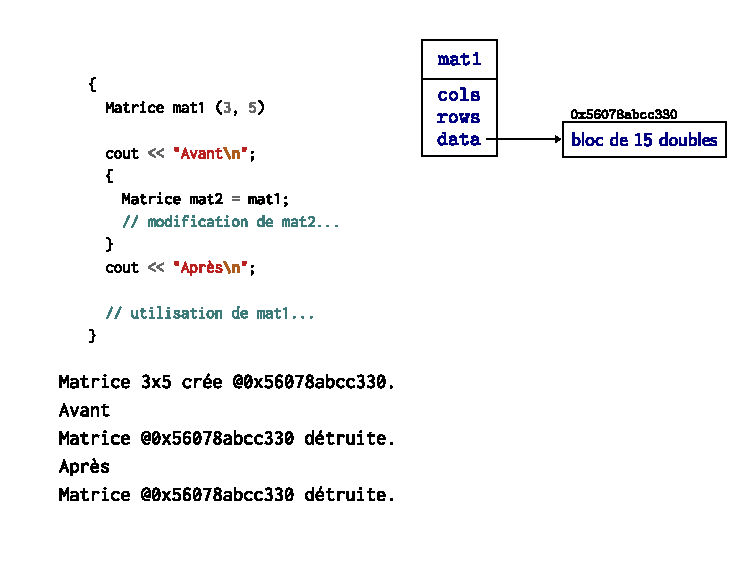
\includegraphics[scale=1]{copiefail1.pdf}
};
\end{tikzpicture}
\end{frame}

\begin{frame}[fragile]{Ça va mal se passer...}
\begin{tikzpicture}[remember picture, overlay]
\node[] at (current page.center) 
{
    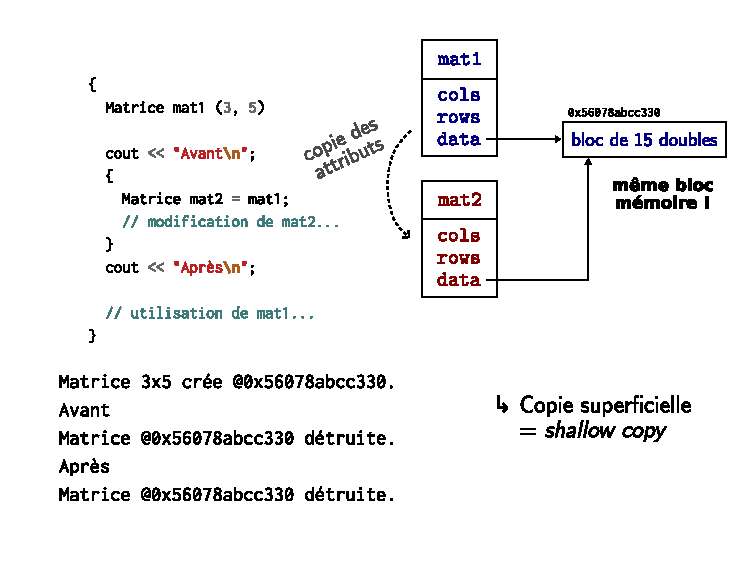
\includegraphics[scale=1]{copiefail2.pdf}
};
\end{tikzpicture}
\end{frame}

\begin{frame}[fragile]{Ça se passe mal}
\begin{tikzpicture}[remember picture, overlay]
\node[] at (current page.center) 
{
    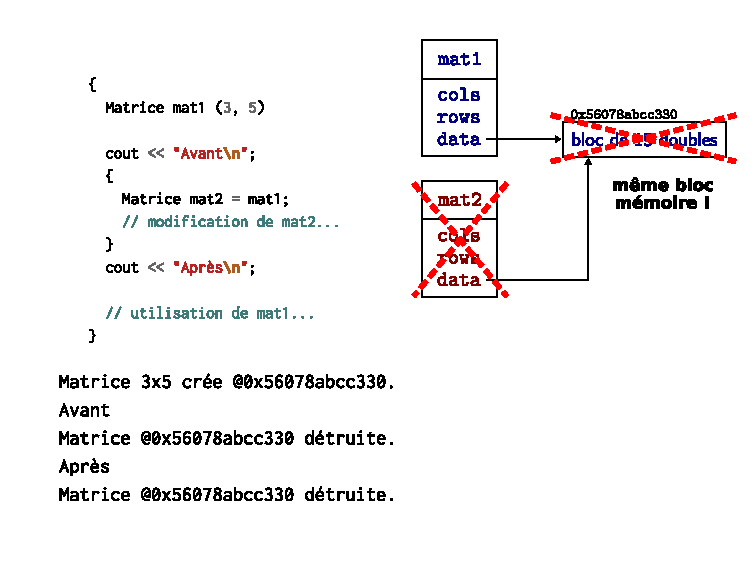
\includegraphics[scale=1]{copiefail3.pdf}
};
\end{tikzpicture}
\end{frame}

\begin{frame}[fragile]{Ça se passe mal}
\begin{tikzpicture}[remember picture, overlay]
\node[] at (current page.center) 
{
    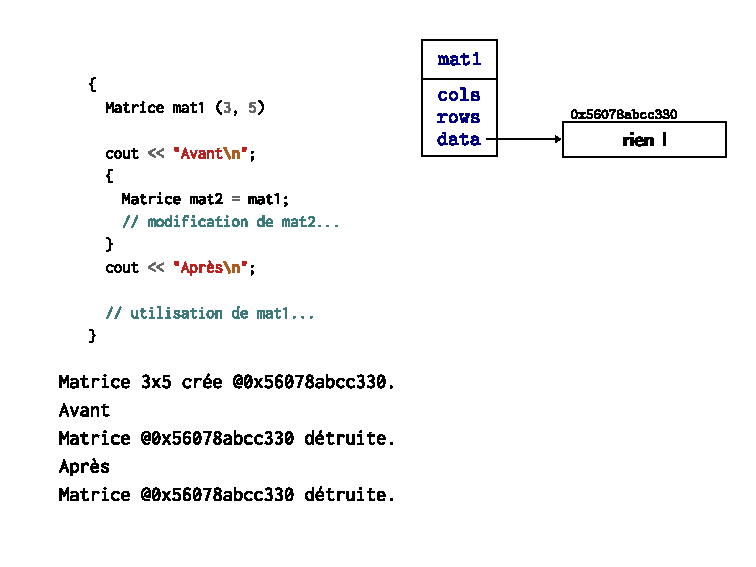
\includegraphics[scale=1]{copiefail4.pdf}
};
\end{tikzpicture}
\end{frame}

\begin{frame}[fragile]{Ce que l'on veut...}
\begin{tikzpicture}[remember picture, overlay]
\node[] at (current page.center) 
{
    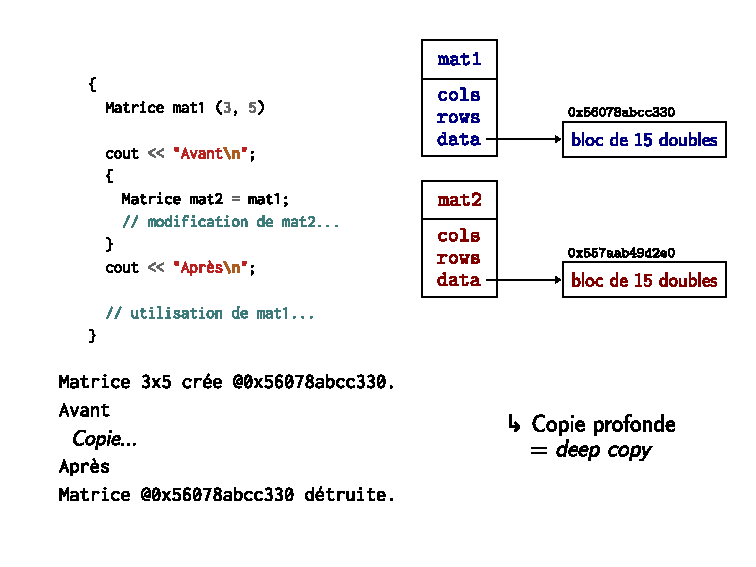
\includegraphics[scale=1]{copiegood1.pdf}
};
\end{tikzpicture}
\end{frame}

\begin{frame}[fragile]{Ça se passe mieux...}
\begin{tikzpicture}[remember picture, overlay]
\node[] at (current page.center) 
{
    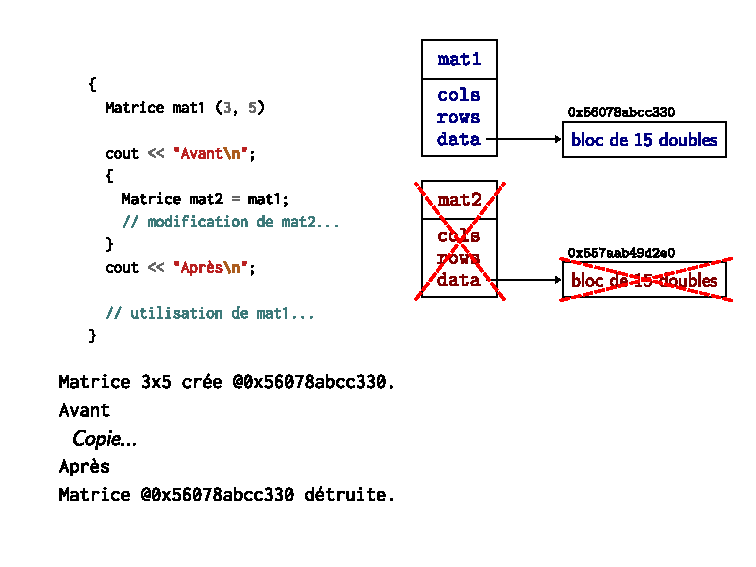
\includegraphics[scale=1]{copiegood2.pdf}
};
\end{tikzpicture}
\end{frame}

%--------------------------------------------------------------------------------------------

\begin{frame}[fragile]{Solution : Constructeur par copie}
  \begin{itemize}
  \item Nécessaire pour effectuer une copie \emph{profonde} (copie contenu mémoire allouée dynamiquement...)
  \item Déclaration :
    \begin{minted}[fontsize=\footnotesize,samepage,mathescape,xrightmargin=0.5cm,xleftmargin=0.5cm]{c++}
      Matrice (const Matrice&);
    \end{minted}
  \item Définition :
    \begin{minted}[fontsize=\footnotesize,samepage,mathescape,xrightmargin=0.5cm,xleftmargin=0.5cm]{c++}
      Matrice::Matrice(const Matrice& other)
        : cols(other.cols), rows(other.rows), data(nullptr)
      {
        data = new double[cols*rows];
        for (unsigned int k = 0; k < cols*rows; k++)
          data[k] = other.data[k];   
      }
    \end{minted}
    \item Utilisation : \texttt{Matrice mat2(mat1);} ou \texttt{Matrice mat2 = mat1;}
    \item Voir exemple dans \texttt{/public/mphyo/M1-C++/TestCopyConstruct}
    \item Alternativement, on peut \emph{interdire la copie} :
    \begin{minted}[fontsize=\footnotesize,samepage,mathescape,xrightmargin=0.5cm,xleftmargin=0.5cm]{c++}
      Matrice (const Matrice&) = delete;
    \end{minted}
  \end{itemize}
\end{frame}

%-----------------------------------------------

\section{Encapsulation}

\begin{frame}[fragile]{Encapsulation : définition}
Encapsulation = interdire/cacher l'accès de certains attributs d'une classe à tout code extérieur à la classe

\begin{itemize}
\item il n'est plus possible d'agir \structure{directement} sur les données d'un objet

\item la modification des attributs de l'objet se fait par \structure{l'intermédiaire de méthodes associées}
\end{itemize}

\structure{Syntaxe :} les mots clés sont \inline{private}, \inline{protected} et \inline{public}
\end{frame}

\begin{frame}[fragile]{Exemple}
\begin{minted}[fontsize=\footnotesize,samepage,mathescape,xrightmargin=0.5cm,xleftmargin=0.5cm]{c++}
class Particule {
private: // facultatif : private par défaut
  // Déclaration des attributs
  double masse_MeV;
  int charge_u;
  ...
};
\end{minted}
\pause
\vspace{1em}
\structure{Conséquence :}
\vspace{1em}
\begin{minted}[fontsize=\footnotesize,samepage,mathescape,xrightmargin=0.5cm,xleftmargin=0.5cm]{c++}
Particule my_kaonplus;
my_kaonplus.masse_MeV = 493.678; // erreur de compilation
\end{minted}
\end{frame}

\begin{frame}[fragile]{Exemple complet (1/2)}
 \begin{minted}[fontsize=\footnotesize,samepage,mathescape,xrightmargin=0.5cm,xleftmargin=0.5cm]{c++}
class Particule {
private:
  // Déclaration des attributs
  double masse_MeV;
  int charge_u;

public:
  // Déclaration des méthodes d'accès
  double get_masse_MeV() const;
  double get_masse_kg() const;
  void set_masse(double masse_MeV_);

  int get_charge_u() const;
  double get_charge_C() const;
  void set_charge(int charge_u_);
};
\end{minted}
\end{frame}

%-----------------------------------------------------------------------

\begin{frame}[fragile]{Exemple complet (2/2)}

\begin{minted}[fontsize=\footnotesize,samepage,mathescape,xrightmargin=0.5cm,xleftmargin=0.5cm]{c++}
// Définition des méthodes
double Particule::get_masse_MeV() const {
  return masse_MeV;
}

void Particule::set_masse(double masse_MeV_) {
  if (masse_MeV_ > 0)
    throw std::range_error("Masse de particule négative !");
  masse_MeV = masse_MeV_;
}

void Particule::set_charge(int charge_u_) {
  if (charge_u_ > 1 or charge_u_ < -1)
    throw std::range_error("Charge de particule doit être -1, 0, ou 1");
  charge_u = charge_u_;
}
...
\end{minted}
\pause
\begin{minted}[fontsize=\footnotesize,samepage,mathescape,xrightmargin=0.5cm,xleftmargin=0.5cm]{c++}
Particule my_kaonplus;
my_kaonplus.set_charge(+1);
double masse = my_kaonplus.get_masse_MeV();
\end{minted}

\end{frame}

%----------------------------------------------------------------------

\begin{frame}[fragile]{Exemple (incomplet) : \texttt{Matrice}}

Il faut interdire l'accès de \texttt{data} à l'utilisateur.
\vspace{1em}
\begin{minted}[fontsize=\footnotesize,samepage,mathescape,xrightmargin=0.5cm,xleftmargin=0.5cm]{c++}
class Matrice {
public:
  ...
  double& operator[](int row, int col);  // Accès à un élément de la matrice

private:
  double* data;
  unsigned int cols, rows;
};
\end{minted}
\pause
\vspace{1em}
\begin{minted}[fontsize=\footnotesize,samepage,mathescape,xrightmargin=0.5cm,xleftmargin=0.5cm]{c++}
double& Matrice::operator[](int row, int col) {
  if (row < 0 or row >= rows or col < 0 or col >= cols)
    throw std::out_of_range();
  return data[ row*cols + col ]; // renvoie une référence
}
\end{minted}
\pause
\vspace{1em}
\begin{minted}[fontsize=\footnotesize,samepage,mathescape,xrightmargin=0.5cm,xleftmargin=0.5cm]{c++}
mat1.accès[1, 2] = 4.2;  // modification via référence
\end{minted}

\end{frame}

%---------------------------------------------------------------------

\begin{frame}[fragile]{Intérêts de l'encapsulation}
\begin{itemize}
\item Lors de la programmation et surtout de la réutilisation d'un objet dans un
autre programme, l'encapsulation empêche la modification non voulue des données
membres

\item L'objet, vu de l'extérieur, \structure{n'est caractérisé que par son \emph{interface}\footnote{c'est à dire l'ensemble des attributs et méthodes effectivement utiles pour l'utilisateur}}\pause :

\begin{enumerate}[<+->]
\item pas d'ambiguïté pour l'utilisateur (\textit{ait-je le droit de modifier cet attribut ?} \textit{est-ce que faire ceci peut faire planter le programme ?}); plus simple; moins d'erreurs
\item la maintenance et l'amélioration de l'objet sont grandement facilitées; tant que la finalité des méthodes et attributs de l'interface publique ne change pas, on peut modifier les rouages sans perturber pour autant les utilisateurs de la classe
\item la classe est facilement réutilisable (cf. héritage)
\end{enumerate}
\end{itemize}
\end{frame}

%----------------------------------------------------

\begin{frame}[fragile]{Intérêts de l'encapsulation}

Règle assez générale :
\begin{itemize}[<+->]
\item \inline{private} si l'attribut doit être protégé
\item Si on envisage qu'un attribut puisse être contraint dans le futur\footnote{en particulier dans une classe fille, cf. cours sur l'héritage} $\rightarrow$ \inline{private}/\inline{protected}
\item Sinon, on \emph{peut} laisser \inline{public}, en particulier si cela évite une lourdeur syntaxique (setters \& getters, ex. : \texttt{vec3}, \texttt{point}...)
\item Dans le doute, préférer \inline{private}/\inline{protected}
\end{itemize}

\end{frame}

%--------------------------------------------------

\part{Affectation \& méthodes spéciales}
\frame{\partpage}

%--------------------------------------------------

\begin{frame}[fragile]{Méthodes spéciales}
Pour l'instant, vous connaissez :
\begin{itemize}
  \item les constructeurs \inline{Classe::Classe(a,b,c,...)}
  \item le constructeur par défaut \inline{Classe::Classe()}
  \item le constructeur par copie \inline{Classe::Classe(const Classe&)} qui sert à créer un nouvel objet à partir d'un objet existant :\\ \inline{Classe b = a;}
  \item le destructeur \inline{Classe::~Classe()}
\end{itemize}
\pause
\vspace{1em}
On peut aussi vouloir assigner un objet à un autre :
\begin{minted}{c++}
Classe b;
...
b = a;
\end{minted}
$\rightarrow$ Assignation par copie
\end{frame}


\begin{frame}[fragile]{Opérateur d'affectation \texttt{=}}
 \begin{itemize}
\item L'opérateur d'affectation \texttt{=} permet d'affecter une nouvelle valeur à un objet \structure{déjà existant} :

\begin{minted}[fontsize=\footnotesize,samepage,mathescape,xrightmargin=0.5cm,xleftmargin=0.5cm]{c++}
Matrice mat1(...);
Matrice mat2(...);
mat2 = mat1;
\end{minted}

\vspace{1em}
\item Sa surcharge se fait comme pour n'importe quel opérateur

\begin{minted}[fontsize=\footnotesize,samepage,mathescape,xrightmargin=0.5cm,xleftmargin=0.5cm]{c++}
// Déclaration
class Matrice {
  ...
  Matrice& operator= (const Matrice& matrice_à_copier);
};
\end{minted}
\end{itemize}
\end{frame}

%------------------------------------------------------------------

\begin{frame}[fragile]{Option n°1}
Parfois, ça se sert à rien, ou ça n'a pas de sens (en particulier lorsque l'objet n'a pas à être copié). On empêche le compilateur de générer des définitions par défaut :\\
\begin{minted}[fontsize=\footnotesize,samepage,mathescape,xrightmargin=0.5cm,xleftmargin=0.5cm]{c++}
class Classe {
  ...
  Classe (const Classe&) = delete;  // construction par copie
  Classe& operator= (const Classe&) = delete;  // assignation
};
\end{minted}
\end{frame}

%------------------------------------------------------------------

\begin{frame}[fragile]{Option n°2}
Si la classe ne contient aucun attribut qui nécessite un traitement spécial ($\neq$ allocation dynamique), on laisse le compilateur copier les attributs de façon naïve :\\
\begin{minted}[fontsize=\footnotesize,samepage,mathescape,xrightmargin=0.5cm,xleftmargin=0.5cm]{c++}
class Classe {
  ...
  Classe (const Classe&) = default;  // construction par copie
  Classe& operator= (const Classe&) = default;  // assignation
};
\end{minted}
\end{frame}

%------------------------------------------------------------------

\begin{frame}[fragile]{Option n°3}
Sinon, pour assigner \inline{obj_b} à \inline{obj_a}, il faut
\begin{enumerate}
  \item détruire ce qui appartenait à \inline{obj_a} (désallocation...)
  \item re-contruire \inline{obj_a} pour accepter le contenu de \inline{obj_b} (allocation...)
  \item copier (en profondeur) le contenu de \inline{obj_b}
\end{enumerate}
\vspace{1em}
\pause
C'est pénible et ça demande de dupliquer du code qui est déjà dans le constructeur par copie, on peut faire des erreurs... Idiome \emph{copy-and-swap} :
\begin{enumerate}[<+->]
  \item copie temporaire de \inline{obj_b} :\\ \inline{Classe obj_temp (obj_b)}
  \item intervertir les attributs de \inline{obj_a} $\leftrightarrow$ \inline{obj_temp}
  \item le compilateur va détruire \inline{obj_temp}, et donc en fait l'ancien contenu de \inline{obj_a}
\end{enumerate}
\end{frame}

\begin{frame}[fragile]{Copy-and-swap en pratique}
\begin{minted}[fontsize=\footnotesize,samepage,mathescape,xrightmargin=0.5cm,xleftmargin=0.5cm]{c++}
class Matrice {
  ...
  ~Matrice();
  Matrice (const Matrice& matrice_à_copier);
  Matrice& operator= (const Matrice& matrice_à_copier);
};

// définition du constructeur par copie
Matrice::Matrice (const Matrice& matrice_à_copier) { ... }

// définition de l'assignation par copie
Matrice& Matrice::operator= (const Matrice& matrice_à_copier) {
  Matrice temp (matrice_à_copier);  // <- copie
  // échange des attributs
  std::swap(cols, temp.cols)
  std::swap(rows, temp.rows)
  std::swap(data, temp.data)
  return *this;
  // <- destruction de temp automatique
}
\end{minted}
\end{frame}


\begin{frame}[fragile]{Copy-and-swap en pratique (encore plus concis)}
\begin{minted}[fontsize=\footnotesize,samepage,mathescape,xrightmargin=0.5cm,xleftmargin=0.5cm]{c++}
class Matrice {
  ...
  ~Matrice();
  Matrice (const Matrice& matrice_à_copier);
  Matrice& operator= (const Matrice& matrice_à_copier);
};

// définition du constructeur par copie
Matrice::Matrice (const Matrice& matrice_à_copier) { ... }

// définition de l'assignation par copie
Matrice& Matrice::operator= (Matrice temp) {
                             // ^- copie
  // échange des attributs
  std::swap(cols, temp.cols)
  std::swap(rows, temp.rows)
  std::swap(data, temp.data)
  return *this;
  // <- destruction de temp automatique
}
\end{minted}
\end{frame}


\begin{frame}[fragile]{Copy-and-swap en pratique}

\begin{minted}[fontsize=\footnotesize,samepage,mathescape,xrightmargin=0.5cm,xleftmargin=0.5cm]{c++}
Matrice mat1 = Matrice(3, 5);
mat1[2,2] = 4.2;
cout << "----------\n";
{
  Matrice mat2 = Matrice(1, 1);
  mat2 = mat1; // assignation par copie
  cout << "mat2[2,2] = " << mat2[2,2] << endl;
}
cout << "----------\n";
cout << "mat1[2,2] = " << mat1[2,2] << endl;
\end{minted}
\pause
\begin{minted}[fontsize=\footnotesize,samepage,xleftmargin=1cm]{text}
Constructeur matrice 3x5 @0x5569ba101eb0.
----------
Constructeur matrice 1x1 @0x5569ba102340.
Constructeur copie matrice 3x5 @0x5569ba102360.
Destructeur @0x5569ba102340.
mat2[2,2] = 4.2
Destructeur @0x5569ba102360.
----------
mat1[2,2] = 4.2
Destructeur @0x5569ba101eb0.
\end{minted}

\end{frame}


%------------------------------------------------------------------

\begin{frame}[fragile]{[À éviter] On pourrait aussi faire...}

\begin{minted}[fontsize=\footnotesize,samepage,mathescape,xrightmargin=0.5cm,xleftmargin=0.5cm]{c++}
class Matrice {
public:
  ...  // déclaration (rappel)
  Matrice& operator= (const Matrice& matrice_à_copier);
private:
  double* data;
  unsigned int cols, rows;
};

// définition de l'assignation par copie
Matrice& Matrice::operator= (const Matrice& matrice_à_copier) {
   if (this != &matrice_à_copier) {  // garde-fou
      if (data != nullptr) delete[] data;  // déallocation
      cols = matrice_à_copier.cols;
      rows = matrice_à_copier.rows;
      data = new double[cols*rows];  // nouvelle allocation
      for (unsigned int k = 0; k < cols*rows; k++)
         data[k] = other.matrice_à_copier[k];  // copie
   }
   return *this;
}
\end{minted}

\end{frame}

%------------------------------------------------------------------

% \begin{frame}[fragile,label={sec:orgheadline9}]{Opérateur d'affectation \texttt{=}}
%  \begin{itemize}
% \item Rien n'empêche toutefois d'affecter un objet à lui-même

% \begin{minted}[fontsize=\footnotesize,samepage,mathescape,xrightmargin=0.5cm,xleftmargin=0.5cm]{c++}
% point my_point;
% my_point = my_point;
% \end{minted}

% \item Lorsque cette ``affectation'' risque de corrompre l'objet, utiliser un
% garde-fou :

% \begin{minted}[fontsize=\footnotesize,samepage,mathescape,xrightmargin=0.5cm,xleftmargin=0.5cm]{c++}
% // Définition
% point & point::operator=(const point & point_)
% {
%   if (&point_ != this) { // garde-fou
%     m_x = point_.m_x;
%     m_y = point_.m_y;
%   }
%   return *this;
% }
% \end{minted}
% \end{itemize}
% \end{frame}

% \begin{frame}[fragile,label={sec:orgheadline10}]{Constructeur de recopie et opérateur d'affectation \texttt{=}}
%  \begin{itemize}
% \item Le constructeur de recopie est la méthode appelée lors de la copie d'un objet
% vers un autre objet du même type

% \begin{minted}[fontsize=\footnotesize,samepage,mathescape,xrightmargin=0.5cm,xleftmargin=0.5cm]{c++}
% int main()
% {
%   point my_vec1(2, 3);
%   point my_vec2 = my_vec1;
% }
% \end{minted}
% \pause
% \begin{minted}[fontsize=\footnotesize,samepage,mathescape,xrightmargin=0.5cm,xleftmargin=0.5cm]{c++}
% class point
% {
%   point(const point & point_);
% };

% point::point(const point & point_)
% {
%   m_x = point_.m_x;
%   m_y = point_.m_y;
% }
% \end{minted}
% \end{itemize}
% \end{frame}

% %---------------------------

% \begin{frame}[fragile,label={sec:orgheadline11}]{Constructeur de recopie et opérateur d'affectation \texttt{=}}
%   \begin{itemize}
%   \item  objets a, b existent avec emplacements dyn. de tailles diff.
    
%   \item affectation \structure{b = a} équivalent à \structure{b.egal(a)} :\\  
    
%     \bigskip
  
%   \item[$\bullet$] \structure{passage de \texttt{a} par valeur}
%     \begin{itemize}
%     \item[-] x (locale) = a // constructeur de recopie nécessaire
%     \item[-] delete b
%     \item[-] new b
%     \item[-] b=x //copie des valeurs des données de x dans b
%     \end{itemize}

%     \bigskip
    
%   \item[$\bullet$] \structure{passage de \texttt{a} par référence}
%     \begin{itemize}
%     \item[-] delete b
%     \item[-] new b
%     \item[-] b=a //copie des valeurs des données de a dans b
%     \end{itemize}

%     \pause
%       \begin{cbox}[6][lbtuc][\centering\small][9][7.5]
%         \ding{42} si a=b OK 
%       \end{cbox}


%        \pause
%       \begin{cbox}[6][lbtuc][\centering\small][9][11]
%         \ding{42} si a=b problème 
%       \end{cbox}
    
%   \end{itemize}
% \end{frame}

% %----------------------------


% \begin{frame}[fragile,label={sec:orgheadline11}]{Constructeur de recopie et opérateur d'affectation \texttt{=}}
%  \begin{itemize}
% \item \Cpp fournit par défaut le constructeur de recopie et l'opérateur
% d'affectation \texttt{=}

% \item Lorsque ces versions triviales ne suffisent pas (cas de \structure{l'allocation
% dynamique}) il faut choisir entre deux solutions :

% \begin{itemize}
% \item Écrire une version correcte (constructeur par copie, surcharge opérateur d'affectation, destructeur)

% \item Rendre impossible la copie et l'affectation, en déclarant ces méthodes
% privées, sans les définir :

% \begin{minted}[fontsize=\footnotesize,samepage,mathescape,xrightmargin=0.5cm,xleftmargin=0.5cm]{c++}
% class pas_de_copie
% {
% private:
%   pas_de_copie(const pas_de_copie&);
%   pas_de_copie & operator=(const pas_de_copie&);
% };
% \end{minted}
% \end{itemize}
% \end{itemize}
% \end{frame}

%------------------------------------------------------------------

\begin{frame}[fragile]{En résumé : deux règles suivant les cas}

\emph{Règle des trois} :\\[0.5em]
Si l'on définit un constructeur qui ouvre une ressource, alloue de la mémoire... ou n'importe lesquelles des méthodes spéciales
\begin{itemize}
  \item[-] Constructeur par copie
  \item[-] Destructeur
  \item[-] Assignation par copie
\end{itemize}
\pause
c'est qu'il faut \textbf{toutes} les définir !\footnote{Définir ne veut pas dire nécessairement les implémenter, lorsque c'est pertinent on peut supprimer la copie ou l'assignation. Pourquoi cette règle ? Eh bien sinon, le compilateur génèrera des méthodes spéciales par défaut qui n'auront pas le bon comportement (copie superficielle).}
\vspace{1em}

\begin{minted}[fontsize=\footnotesize,samepage]{c++}
class Classe {
  Classe (...);  // constructeurs
  Classe (const Classe&);  // constructeur par copie
  Classe& operator= (const Classe&);  // assignation par copie
  ~Classe();  // destructeur
};
\end{minted}

\end{frame}


\begin{frame}[fragile]{En résumé : deux règles suivant les cas}

\emph{Règle du zéro} :\\[0.5em]
Utiliser au maximum les objets de bibliothèques existantes (\inline{std::vector}, \inline{std::string}) et éviter l'allocation manuelle de mémoire. On peut alors laisser le compilateur implémenter toutes les méthodes spéciales par défaut !
\vspace{1em}

\begin{minted}[fontsize=\footnotesize,samepage]{c++}
class Classe {
  Classe (...);  // constructeurs
  Classe (const Classe&) = default;
  Classe& operator= (const Classe&) = default;
  // pas de destructeur
};
\end{minted}

\end{frame}

%---------------------------------------------------------------

\part{Et dans d'autres langages ?}
\frame{\partpage}

\begin{frame}[fragile]{Et dans d'autres langages ?}

La notion d'objets est présente dans de nombreux langages, y compris Python, Java, OCaml... C'est surtout au niveau de la gestion de la mémoire, de la construction/destruction, de la copie... que se trouvent les différences.\\

En Python, la notion de constructeur existe, mais la notion de destruction ou de copie ne peut être calquée sur le \Cpp. En effet, le moment où l'objet est effectivemet détruit est non déterministe. Pas de \inline{const} non plus.\\

\end{frame}

\begin{frame}[fragile]{Petit exemple en Python}

\begin{minted}[fontsize=\footnotesize,samepage]{python}
class Point:
  def __init__(self, x=0, y=0):  # constructeur
    self.x = x
    self.y = y

  def __add__(self, other):
    return Point(self.x + other.x, self.y + other.y)

  def norme(self):
    return (self.x**2 + self.y**2) ** 0.5

  def afficher(self):
    print(f"({self.x}, {self.y})")

p = Point(1.5, 2.0)
import copy
p2 = copy.copy(p)  # la copie doit être explicite
# si non utilisés, ces deux objets seront détruits un jour...
# mais il est possible de forcer la chose :
del p
\end{minted}

\end{frame}

%---------------------------------------------------------------

\part{Déplacer au lieu de copier}
\frame{\partpage}

\begin{frame}[fragile]{Exemple de copie évitable}
Mais on peut souvent éviter des copies inutiles :

\begin{columns}
\begin{column}{0.5\columnwidth}
\begin{minted}[fontsize=\footnotesize,samepage,mathescape,xrightmargin=0.5cm,xleftmargin=0.5cm]{c++}
Matrice f () {
  Matrice mat (3000, 5000);
  return mat;
}
\end{minted}

\begin{cbox}[][lwuc][\centering\footnotesize]
La variable locale \texttt{mat} est copiée dans un objet anonyme retourné par la fonction.
\end{cbox}

\end{column}
\begin{column}{0.5\columnwidth}
\begin{minted}[fontsize=\footnotesize,samepage,mathescape,xrightmargin=0.5cm,xleftmargin=0.5cm]{c++}
Matrice f () {
  return Matrice(3000, 5000);
}
\end{minted}

\vspace{0.7em}

\begin{cbox}[][lwuc][\centering\footnotesize]
Il n'y a plus de variable locale. L'objet anonyme est construit directement.
\end{cbox}
\end{column}
\end{columns}

\vspace{1.5em}
\pause
Le compilateur est souvent capable d'effectuer ces optimisations automatiquement, mais mieux vaut prendre des bonnes habitudes. Cependant, ça n'est parfois pas possible, et le compilateur peut ne pas voir certaines optimisations. On peut l'aider...

\end{frame}

%-------------------------------

\begin{frame}[fragile]{Move semantics}
Dans le \Cpp11, un nouveau concept a été introduit : le déplacement d'objets (\textit{move semantics}). L'objectif est de gagner en performances en évitant les copies inutiles. Ainsi qu'en permettant le déplacement d'un objet même lorsque la copie n'a pas de sens. Par exemple, lors d'un retour de fonction :
\begin{minted}[fontsize=\footnotesize,samepage,xrightmargin=0.5cm,xleftmargin=0.5cm]{c++}
std::vector<int> ma_fonction () {
  std::vector<int> vec;
  ...
  return vec;
}

...
std::vector<int> resultat = ma_fonction();
\end{minted}
le compilateur va \emph{déplacer} \texttt{vec} dans \texttt{resultat}, au lieu d'appeller le constructeur par copie de \inline{std::vector<int>}.
\end{frame}

\begin{frame}[fragile]{Move semantics}
Pour cela, le \Cpp11 a introduit les \textit{rvalue references} (que l'on pourrait traduire par "référence de valeur à droite d'une égalité"), par opposition aux usuelles \textit{lvalue references}. Une \textit{rvalue references} d'un type \inline{Type} se note \inline{Type&&}.\\

Il existe alors deux nouvelles méthodes spéciales : le constructeur par déplacement, et l'assignation par déplacement :
\begin{minted}[fontsize=\footnotesize,samepage]{c++}
class Classe {
  Classe (...);  // constructeurs
  Classe (const Classe&);  // constructeur par copie
  Classe& operator= (const Classe&);  // assignation par copie
  Classe (Classe&&);  // constructeur par déplacement
  Classe& operator= (Classe&&);  // assignation par déplacement
  ~Classe();  // destructeur
};
\end{minted}
qui seront appelés à la place de celles par copie lorsque l'objet de droite est une \textit{rvalue references}.
\end{frame}

\begin{frame}[fragile]{Move semantics}
Exemple :
\vspace{1em}
\begin{minted}[fontsize=\footnotesize,samepage]{c++}
Classe c1 (...);

Classe c2 = c2; // constructeur par copie

Classe c3 = std::move(c1); // constructeur par déplacement
\end{minted}
\vspace{1em}
Ici, \inline{c1} est déplacé dans \inline{c3}, et non copié. Attention, après cette opération, \inline{c1} ne doit plus être utilisé !
\end{frame}

%--------------------------------------------------------------

\begin{frame}[fragile]{Move semantics}
Exemple avec \inline{Matrice} :
\vspace{1em}
\begin{minted}[fontsize=\footnotesize,samepage]{c++}
// Définition du constructeur par déplacement
Matrice::Matrice (Matrice&& mat_à_déplacer)
  // on "vole" les attributs de `mat_à_déplacer`
  : cols(mat_à_déplacer.cols),
    rows(mat_à_déplacer.rows),
    data(mat_à_déplacer.data)
{
  // on laisse `mat_à_déplacer` dans un état valide :
  mat_à_déplacer.cols = 0;
  mat_à_déplacer.rows = 0;
  mat_à_déplacer.data = nullptr;
}
\end{minted}
\vspace{1em}
Déplacer un objet, ce n'est rien d'autre que \emph{voler ses attributs} tout en laissant derrière soi un état valide
\end{frame}

\begin{frame}[fragile]{Move semantics}
Lorsque la classe ne contient que des attributs qui n'ont pas besoin de traitement spécial (fermeture de ressource, désallocation...), on peut laisser le compilateur le définir par défaut :
\begin{minted}[fontsize=\footnotesize,samepage,xrightmargin=0.5cm,xleftmargin=0.5cm]{c++}
class Classe {
  Classe (...);  // constructeurs
  Classe (Classe&&) = default;  // constructeur par déplacement
  Classe& operator= (Classe&&) = default;  // assignation par déplacement
};
\end{minted}
Le compilateur les génèrera automatiquement si il n'y a pas de destructeur de défini.
\end{frame}

%--------------------------------------------------------------

\begin{frame}[fragile]{Move semantics}
Cas d'utilisation :
\begin{itemize}
  \item On peut vouloir stocker des objets de type \inline{Classe}, non copiables (par exemple représentant une ressource physique), dans un \inline{std::vector<Classe>}. C'est possible, mais seulement si le constructeur par déplacement est défini.
  \item \inline{std::sort()} passe sa vie à échanger des éléments dans un tableau pour le trier : ça sera beaucoup plus efficace si constructeur par déplacement est défini !
  \item Lorsque les types des attributs utilisés sont élémentaires (\inline{int}, \inline{double}...), ça ne sert à rien
  \item Ça reste une notion complexe et avancée qu'il n'est pas du tout nécessaire de maîtriser ni même de connaître
\end{itemize}
\end{frame}

\end{document}
